%!TeX program = pdfLaTeX
\documentclass[11pt,twocolumn]{article}
\usepackage[AutoFakeBold=true, AutoFakeSlant=true]{xeCJK}
\usepackage[utf8]{inputenc}
\usepackage{lipsum}
\usepackage[margin=1in]{geometry}
\usepackage{graphicx}
\usepackage{adjustbox}
\usepackage{hyperref}
\usepackage{fontspec}
\setmainfont{Times New Roman}
\setCJKmainfont{cwTeXMing}
\usepackage{multicol}
\usepackage{indentfirst}
\setlength{\columnsep}{1cm}
\usepackage{natbib}
\usepackage{graphicx}
\usepackage{makecell}
\renewcommand{\figurename}{圖}
\renewcommand{\tablename}{表}
\renewcommand{\refname}{參考文獻}
\usepackage[linesnumbered,ruled,vlined]{algorithm2e}
\renewcommand{\algorithmcfname}{演算法}
\pagenumbering{gobble}

\title{
分散式資料庫增加資料儲存安全性之方法研究\\
Method of securely storing data in distributed databases
}
\author{
  張睿玹*\\
  \texttt{TNFSH}\\
  \texttt{hsuan@hsuan.app}
  \and
  鄭弘煒\\
  \texttt{TNFSH}\\
  \texttt{wei@sivir.pw}
}

\date{February 2021}

\begin{document}

\maketitle
\section*{摘要}
本研究擬改善現存儲存機敏資料技術,發展更加安全的儲存技術。\par
首先,本研究提出透過中心化分散式資料庫、加密算法等技術,提出一種安全地儲存機敏資料的方法,透過這個方法,可以在有效率、安全的狀況下儲存資料,接著使用Docker、Flask等技術實作出此套系統,最終透過壓力測試,將傳統儲存機敏資料的方式與本研究提出之儲存方式進行比較,驗證本研究提出之儲存方式確實為一有效率之方法。\par
最後,本研究希望透過改良儲存方法,增加資料安全性,確保網路上所流通之機敏資料不被攻擊者所獲。

\textbf{關鍵詞:} 分散式資料庫;雲端儲存;資料安全

\section*{Abstract}
The research was devoted to improving the existing data storing techniques and develop a more secure data storing technique than before.\par
First, the research proposed a method to securely store secret data using centralized management of distributed databases and encryption algorithm.\par
With this method, people can store data efficiently and securely.We use Docker and Flask to implement the proposed system. Through the stress tests, we proved that storing in the proposed system was more efficient than in the original one.\par
Finally, the research hopes to increase data security and ensure the secret data on the Internet won't be revealed.

\textbf{Keywords:} distributed database system;cloud storage;data security

\section{緒論}
\subsection{研究動機}
現今的網頁程式在資料儲存時大多使用後端程式搭配SQL資料庫,倘若後端程式寫的不夠嚴謹,造成諸如SQL Injection、Arbitrary File Download之網頁漏洞,攻擊者如果能輕易取得這些資料庫中的內容,都可能造成各種資訊外洩的風險,在這網路如此發達、各個網站上都存放了許多機敏的個人資料時代,是個極大的危機。\par
網際網路存取十分方便,卻也間接導致人們過於依賴網路、深信著網路世界的安全。在網路爆炸的年代,各公司遭受駭客的侵擾時有所聞,可見,不論電腦再怎麼持續的更新,依然會有資安漏洞存在。但如果將資料透過加密,並且分散地儲存在系統之中,除了不會影響到資料讀取的方便性,同時也能讓攻擊者取得資料後更難將其還原,降低了資料外洩的隱憂。\par
本研究擬改善現有儲存資料的方式,以更加安全、犧牲最少使用者利益的方式儲存機敏資料,期待為資訊安全領域貢獻心力。\par

\subsection{研究目的}
本研究目的為確保網路上儲存之使用者資料安全性,自現行的資料儲存技術中再做調整,研究如何達到更高的安全性。\par
\begin{enumerate}
  \item 研究避免單一資料庫遭攻擊造成資料外洩之方法
  \item 設計兼顧安全性及穩定性,且易部署、易整合之資料儲存系統
\end{enumerate}


 
 
\section{相關研究}
\subsection{分散式儲存系統及分散式資料庫}
有別於一般的傳統關聯式資料庫,分散式資料庫系統會在許多不同的地點設置資料庫中心,並在所有的資料庫中存放著相同的檔案,如此,在使用者請求後,可以從任意一個伺服器下載,以提升速度並降低延遲。但有同時亦有缺點,資料儲存在多個伺服器中,只要一個伺服器遭駭後,檔案資料便會遭到外洩,資料保密性和安全性便受到不小威脅。\par
研究者利用分散式儲存系統多伺服器的特性並加以改良,始得此研究之初始想法。\par

\cite{centralDDBMS}中提出分散式資料庫中心化管理方式,本研究中的分散式資料庫管理系統即與其精神十分相似,利用中心化的管理技術方便地管理分散式資料庫中的資料。\par
\cite{distributed_filesystem}以GlusterFS和Docker等開放原始碼軟體建置雲端儲存服務,GlusterFS乃一分散式儲存系統,其特性之之一:不必建置metadata伺服器,而是以演算法算出資料儲存之位置,在其研究中,運行之效率皆在可接受之範圍內,可見分散式儲存系統乃一可商業使用之技術。\par
\cite{DISCO}開發一支援OpenStack之分散式儲存系統,其系統具備完善的功能,且會將資料進行備份,也加入多種技術來提高資料儲存效率。\par

\subsubsection{資料安全}
資料安全乃為當代十分重要的議題,雲端儲存服務商除了在確保商業利益外,更應注重使用者的資料安全。\par
\cite{clouddatasafe}指出現今雲端儲存服務快速發展,保障資料安全變成一個艱困的議題,並實作一個針對現有服務的檔案加密系統,藉此保障使用者的資訊安全。

\section{系統架構}

\begin{figure}[h]
\centering
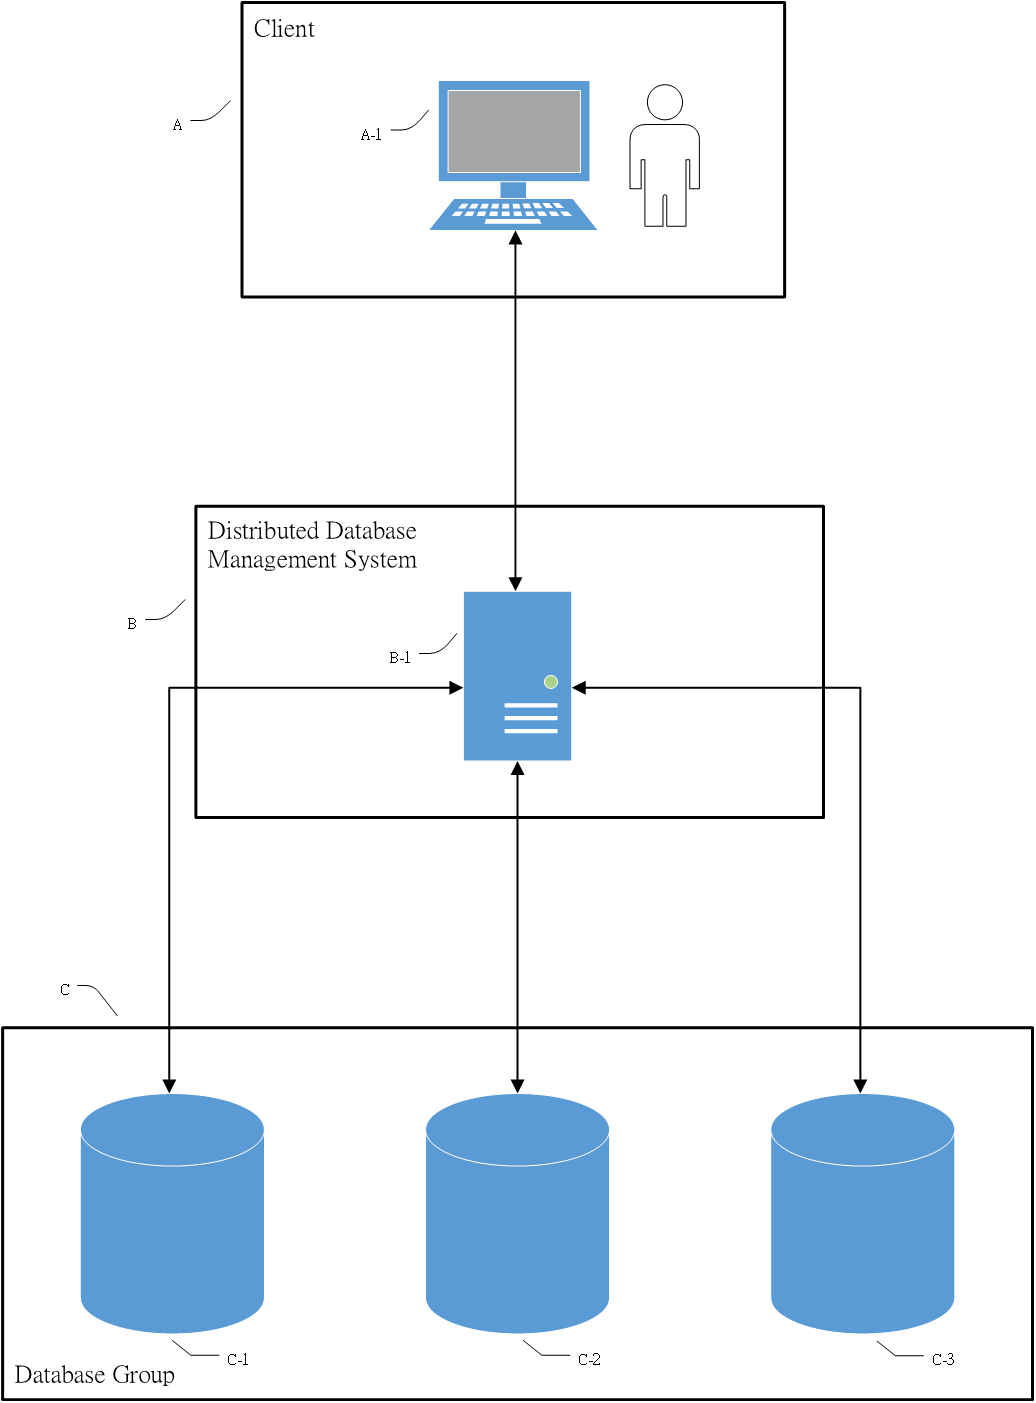
\includegraphics[scale=0.3]{Fig.1.png}
\caption{系統架構圖}
\end{figure}

\subsection{架構設計}
本研究提出一系統 (見圖 1),其主體乃一分散式資料庫,整個系統共包含: 用戶端、分散式資料庫管理系統(以下簡稱DDBMS)、資料庫群,互相透過網路進行溝通。\par
與其他同為分散式資料庫之系統不同,本系統並非額外使用資料庫儲存資料存放之位置,而是使用自行設計之資料分割演算法,只要透過儲存時所使用之客戶端傳送的金鑰就可以存取資料。\par
用戶端可為任一具發送HTTP請求之服務,負責與DDBMS溝通。分散式資料庫管理系統負責管理各個資料庫,當接收到儲存資料的訊號時,依照編寫的演算法(見演算法1)將資料安全的儲存至不同的資料庫中。資料庫群則是由多個資料庫組合而成,透過獨立的區域網路分別與上述之分散式資料庫管理系統溝通。\par
\subsubsection{Client 用戶端}
此安全之儲存方法可應用於各種場景,使用者體驗與一般儲存方法無異。用戶端可以任何程式語言開發,惟必須透過HTTP請求與本研究設計之系統主體——DDBMS溝通,透過DDBMS來存取、加解密位於資料庫中的資料。\par

\subsubsection{Distributed Databases Management System 分散式資料庫管理系統}

DDBMS是本系統的關鍵服務,其工作為與客戶端溝通,並操作資料庫群,在存取的時候,加入了加解密的步驟,提高資料的安全性。\par
在收到存取資料庫的信號後,DDBMS會將收到的金鑰和內容透過設計的分割資料演算法去做處理(見 3.1.4)。\par
DDBMS提供了API供客戶端與之溝通,提供讀取、寫入資料之操作介面。\par
\subsubsection{Database Groups 資料庫群}
Database Group是一群資料庫,透過DDBMS統一存取,其中每個Database都使用了MySQL Cluster技術,避免單一資料庫故障,全部的資料皆無法存取。\par
DBGroup中的資料庫格式如下表,每一個位於MySQL-cluster中的node都會有下表所示之資料庫:\par

\begin{table}[h]
    \centering
    \begin{tabular}{ |c|c|c| }
     欄位名稱 & 資料型態 & 欄位內容 \\
     \hline
     tag & varchar(36) & 資料標籤 \\ 
     data & longtext & 資料內容
    \end{tabular}
    \caption{DBGroup資料庫格式}
\end{table}

\subsubsection{分割資料演算法}
此研究藉由將資料分割、加密,以期提高資料儲存的安全性。\par
在本研究設計的演算法中,共有兩個需要輸入給DDBMS的參數: 欲儲存的內容、金鑰,以及一個可在系統初始化時設定的常數: 資料庫數量。\par
首先,本系統會將輸入的資料內容透過base64編碼成文字,避免資料內容是二進位檔案時,直接操作byte造成不必要的問題。而後研究者發現如果單純使用base64儲存,縱使將資料分割到不同的資料庫儲存,任一資料庫若被攻破,攻擊者得到部分編碼後的資料,仍是有可能回推部分資料的,因此,研究中加入了加密函式,將資料先行加密,改成儲存密文,如此一來,縱使有部分資料被攻擊者取得,也無法順利回推資料內容。\par
客戶端會傳送一個金鑰給DDBMS,在本研究所提出之範例系統中,以使用者的UUID作為此金鑰,將此金鑰透過Hash函式得到一個固定長度的Hex字串MapKey(演算法1第2行),藉由此字串作為儲存到資料庫時的Mapping。由於環境不同,有些環境可能資源較少,Database Group中只有少數幾台,若依照原先的演算法,在存放資料時會有影響,可能會發生資料無法存完的問題,因此研究者想到一個解決辦法,取Hash的前n個字,這個n代表資料庫的數量,這樣一來在處理儲存的動作時就不會受到影響。(參考圖2)\par
接著透過這個Hash過的Key作為Mapping,先遍歷每個在MapKey中的字元,透過函式SplitLength得出該區間應該切的長度,並將資料切割,再依序存到資料庫中。\par
\begin{algorithm}
	\caption{
	    資料分割演算法
	}\label{algo:b}
		
	\SetKwInOut{Input}{Input}
	\SetKwInOut{KwOut}{Output}  
	\SetKwInOut{KwData}{Data}  
		
	\Input {
		$content$: 欲儲存的內容\\
		$key$: 金鑰\\
		$n$: 資料庫數量
	}
	\KwData {
		0 $<$ SplitLength(c) $\leq$ 1 將字元c轉成要切的長度
	}
	
	content $\gets$ encrypt(base64(content),key) \;
	map\_key $\gets$ hash(key)[0:n] \;
		
	last $\gets$ 0\;
		
	\For{index $i$, character $c$ of $map\_key$}{
		len $\gets$ $length$(content) * $SplitLength$(c)\;
		$SaveToDatabase$(i, content[last+1:last+len])\;
		last $\gets$ last + len\;
	}
\end{algorithm}
\subsubsection{SplitLength函式運作原理}
SplitLength函式會存取一個config檔案,這個檔案是在程式初始化的時候,就設定好的,因此在每個系統實例中,若輸入SplitLength的字元相同,就會得到相同數值,藉此確保使用者資料能夠正常還原,透過這個數值,將原本要儲存的資料依序切成不同長度,再依序存到資料庫中,在取出時亦然,依序從資料庫中取出資料,合併再還原成原本的資料回傳給使用者。\par
\begin{table}[h]
    \centering
    \begin{tabular}{ c }
    \hline
    a 0.75\\
	b 0.54\\
	c 0.53\\
	d 0.54\\
	e 0.54\\
	f 0.35\\
	0 0.79\\
	1 0.61\\
	2 0.69\\
	3 0.44\\
	4 0.22\\
	5 0.13\\
	6 0.71\\
	7 0.53\\
	8 0.38\\
	9 0.36\\
	\hline
    \end{tabular}
    \caption{SplitLength config檔案}
\end{table}

\begin{figure}[h]
\centering
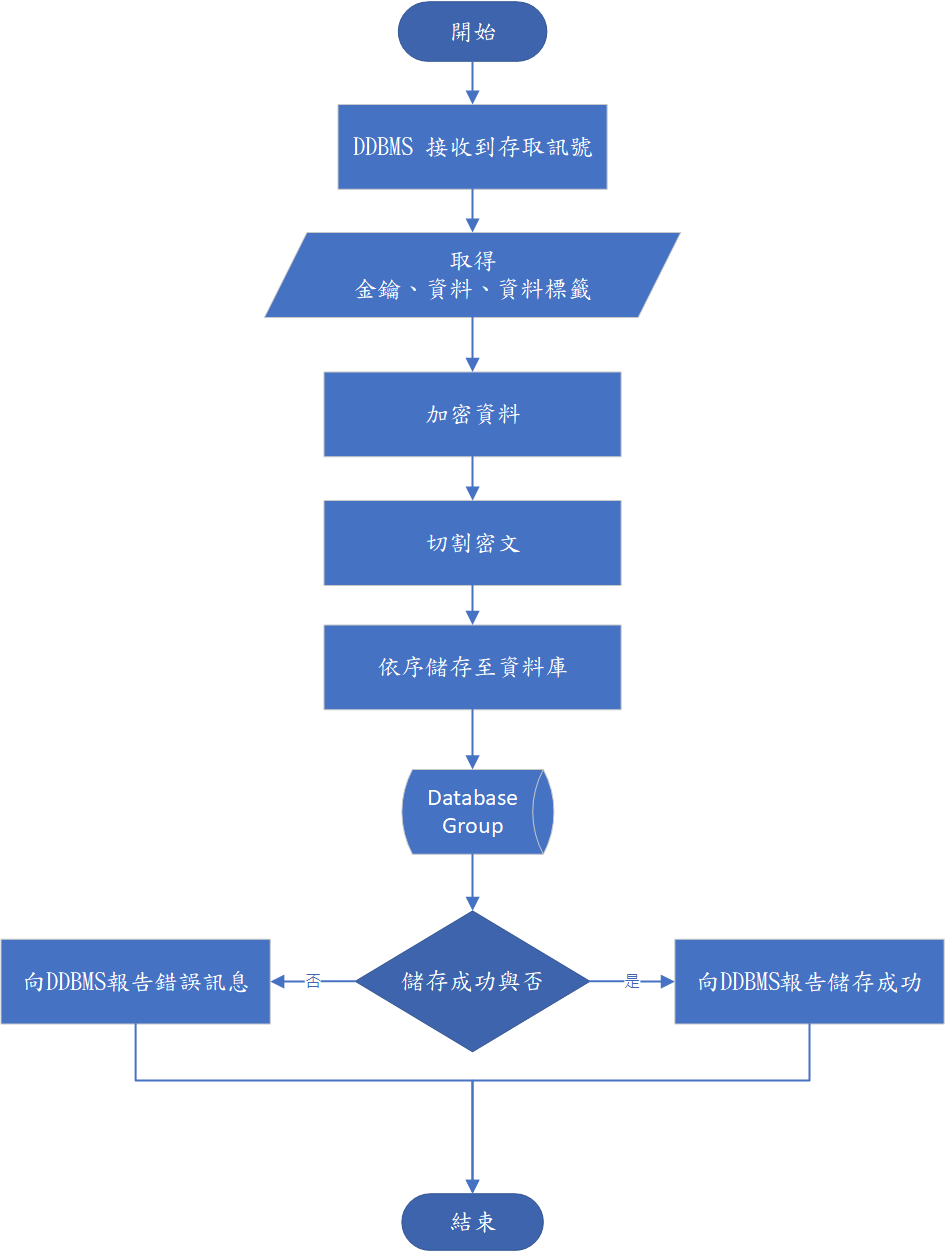
\includegraphics[scale=0.4]{Fig.2.png}
\caption{儲存流程圖}
\end{figure}

\subsection{系統特色}
本作品著重於DDBMS之設計,透過提供API endpoint,讓不同架構的程式也能與之溝通,本研究中利用當今十分常見的Laravel (PHP) + HTML實作出簡易檔案上傳管理系統,並將此研究中的系統Docker化,因此在部屬上亦十分容易就能將整個系統建置好,並完成整合。
\newpage
\section{研究結果}
\subsection{系統安全性}
\begin{figure}[h]
\centering
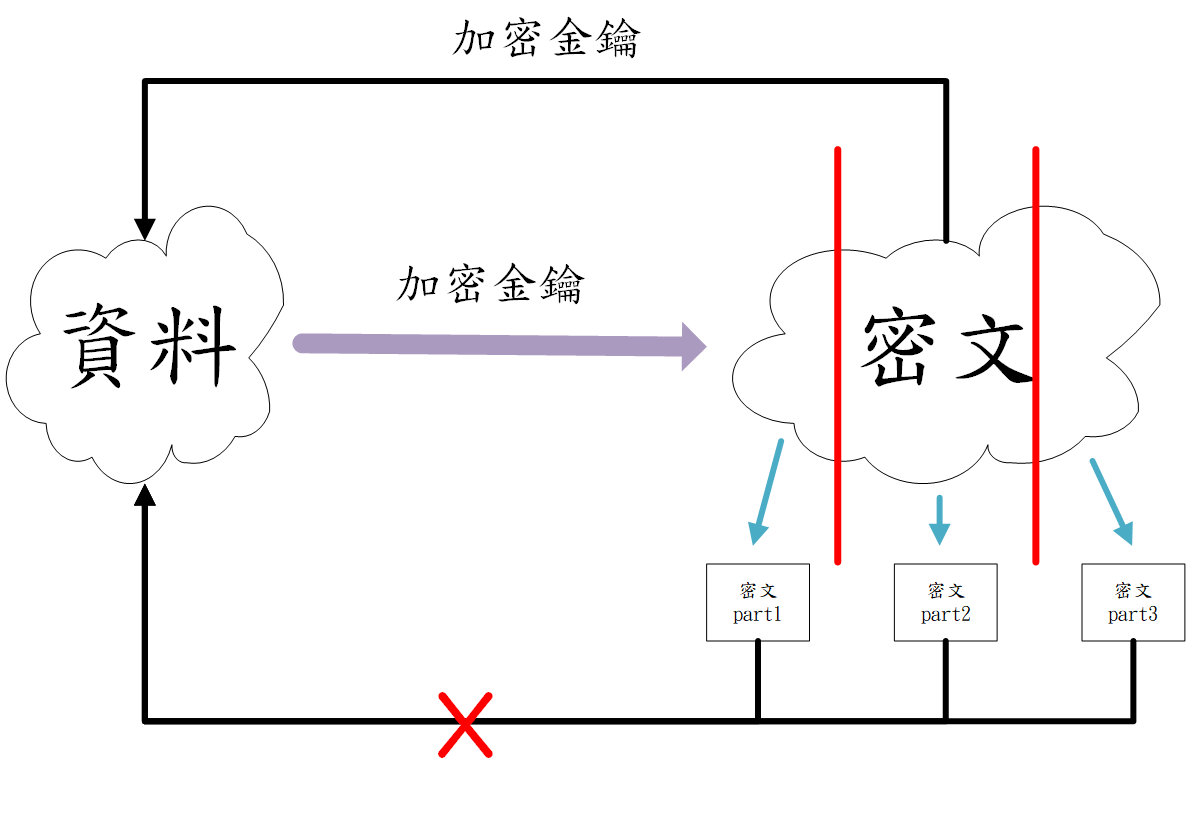
\includegraphics[scale=0.3]{Fig.3.png}
\caption{加解密概念圖}
\end{figure}

此研究設計的這套系統在儲存資料時,將資料加密再分割,研究者當初即是想到現今網路攻擊氾濫,當儲存資料的單一資料庫遭攻擊,資訊就會直接外洩。(見圖3)\par
將資料分割的好處是攻擊者取得單一資料庫內容後,沒辦法得知原始的內容,但後來我們發覺此方法仍有資料外洩之可能,因此引入了加密算法,先將資料加密,且非整個系統都採用相同金鑰,而是每個使用者的金鑰皆不同,縱使是單一資料庫外洩時,也能確保原始訊息的安全,惟所有資料庫都被攻破、且攻擊者已取得每則資料加密之金鑰時,存於資料庫中的資料才會外洩,不但要將多個資料庫都攻破之難度極高、且必須拿到每個使用者皆不同的金鑰進行解密,為了達成此攻擊,不但時間成本極高,所需之經費亦十分高,並不符合正常攻擊者的利益。

\subsection{系統性能分析}

透過壓力測試,取得效能之數據,並加以分析。
此研究將原始儲存方式作為對照組(將資料加密後存入資料庫),將設計之系統作為實驗組,透過壓力測試,進行數據分析。

\subsubsection{多人連線檔案連續傳輸}
以不同上線人數上傳100個請求,比較本系統之處理效能(單位: 毫秒ms)\par
(參考表3、圖4)\par
\begin{table*}[ht]
    \centering
    \begin{tabular}{ |c|c|c|c|c|c|c| }
    \hline
    \thead{Percentage}  & \thead{對照組\\1人上線} & \thead{實驗組\\1人上線} & \thead{對照組\\10人上線} & \thead{實驗組\\10人上線} & \thead{對照組\\100人上線} & \thead{實驗組\\100人上線} \\
   \hline
50\% & 108 & 125 & 289 & 453 & 4449 & 4410\\
66\% & 123 & 141 & 325 & 474 & 4890 & 4810\\
75\% & 125 & 149 & 504 & 487 & 5149 & 5132\\
80\% & 132 & 156 & 691 & 490 & 5272 & 5332\\
90\% & 153 & 186 & 1238 & 507 & 5610 & 5699\\
95\% & 203 & 308 & 1965 & 535 & 5752 & 5957\\
98\% & 391 & 572 & 2024 & 638 & 6895 & 6066\\
99\% & 1176 & 1182 & 2064 & 801 & 7000 & 6160\\
100\% & 1176 & 1182 & 2064 & 801 & 7000 & 6160\\
    \hline
    \end{tabular}
    \caption{多人連線檔案連續傳輸時間統計}
\end{table*}

\begin{figure}[h]
\centering
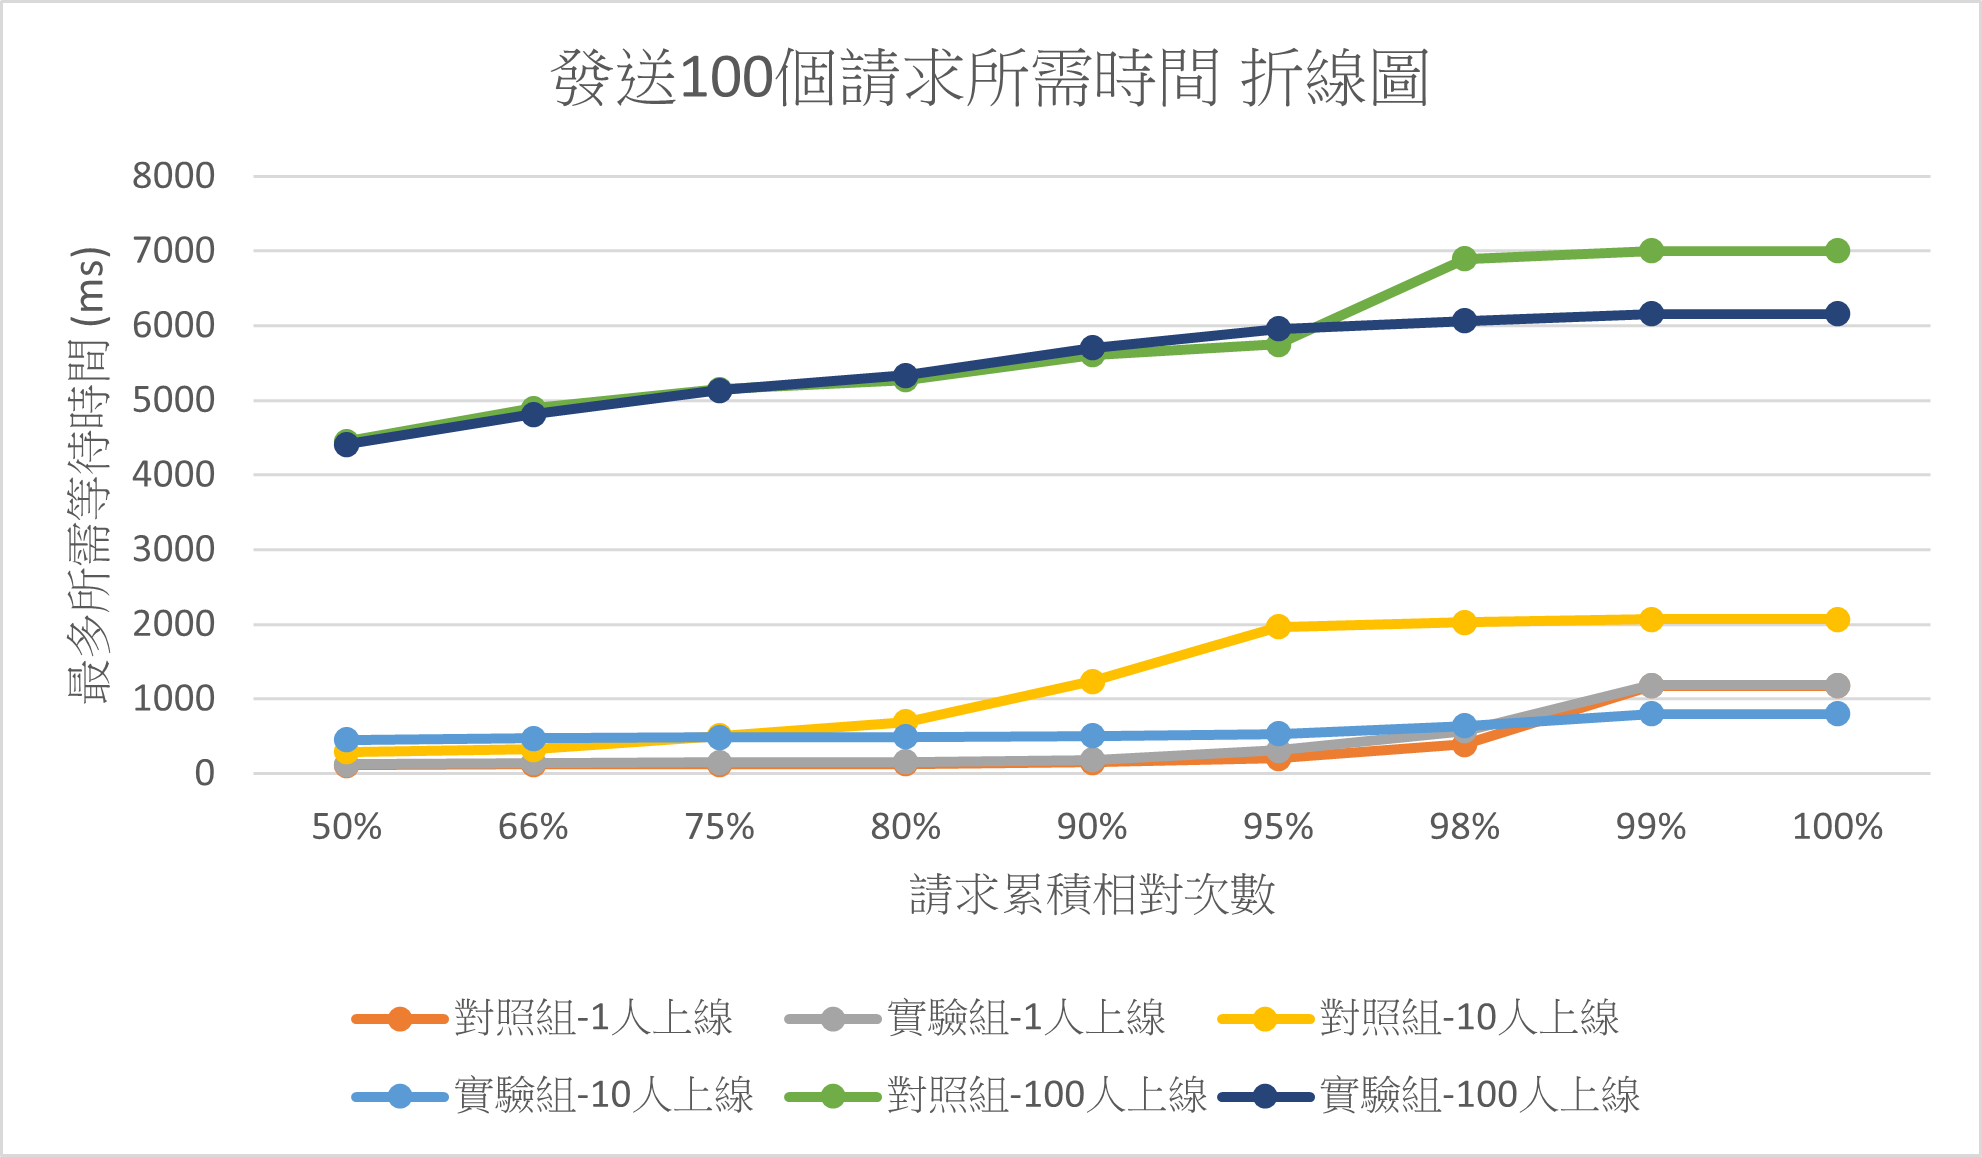
\includegraphics[scale=0.5]{多人連線檔案連續傳輸耗時折線圖}
\caption{多人連線檔案連續傳輸耗時折線圖}
\end{figure}
從上述資料可以發現:在每次的實驗中,對照組比實驗組還需要花多一些的時間來處理資料,且相對而言,實驗組所需的時間較為穩定,最久的等待時間和最短的等待時間相差不多,不會造成有些使用者很快,有些使用者很慢的問題。\par
\newpage
\subsubsection{20MB檔案上傳耗時}
透過壓力測試,測試上傳20MB檔案所需時間,共測30次,取其平均,並將數據進行分析。(單位: 毫秒ms)\par
(參考圖5、圖6、圖7)
\begin{figure}[h]
\centering
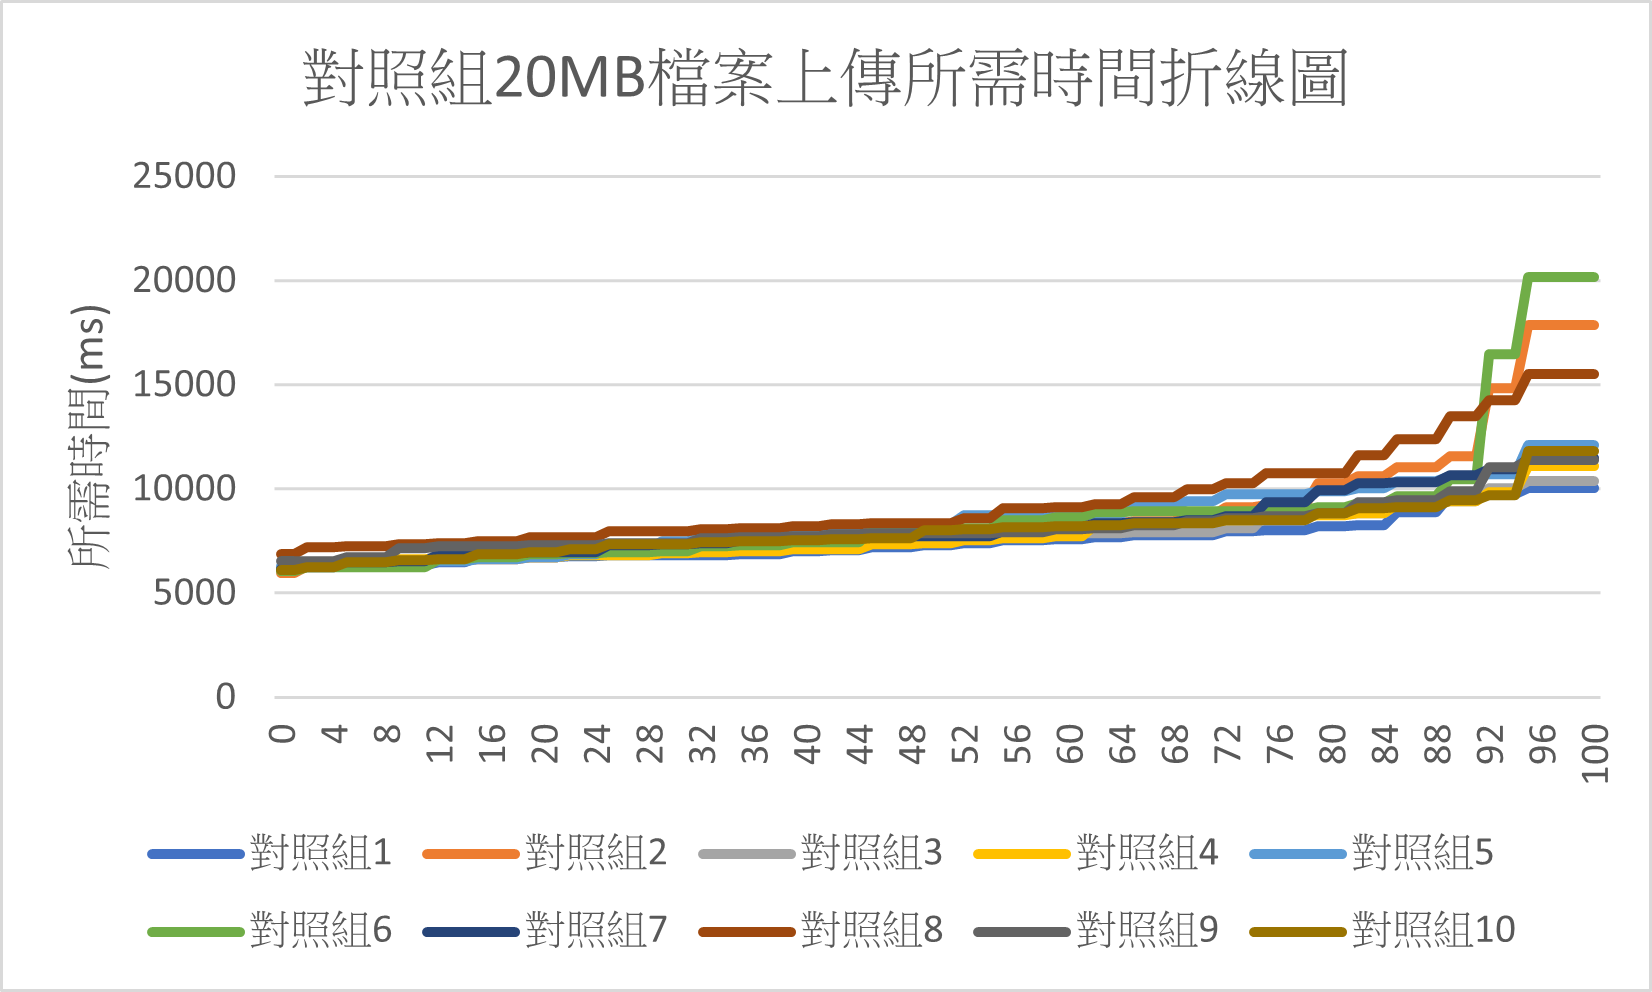
\includegraphics[scale=0.55]{對照組20MB檔案上傳所需時間折線圖.png}
\caption{對照組20MB檔案上傳所需時間折線圖}
\end{figure}

\begin{figure}[h]
\centering
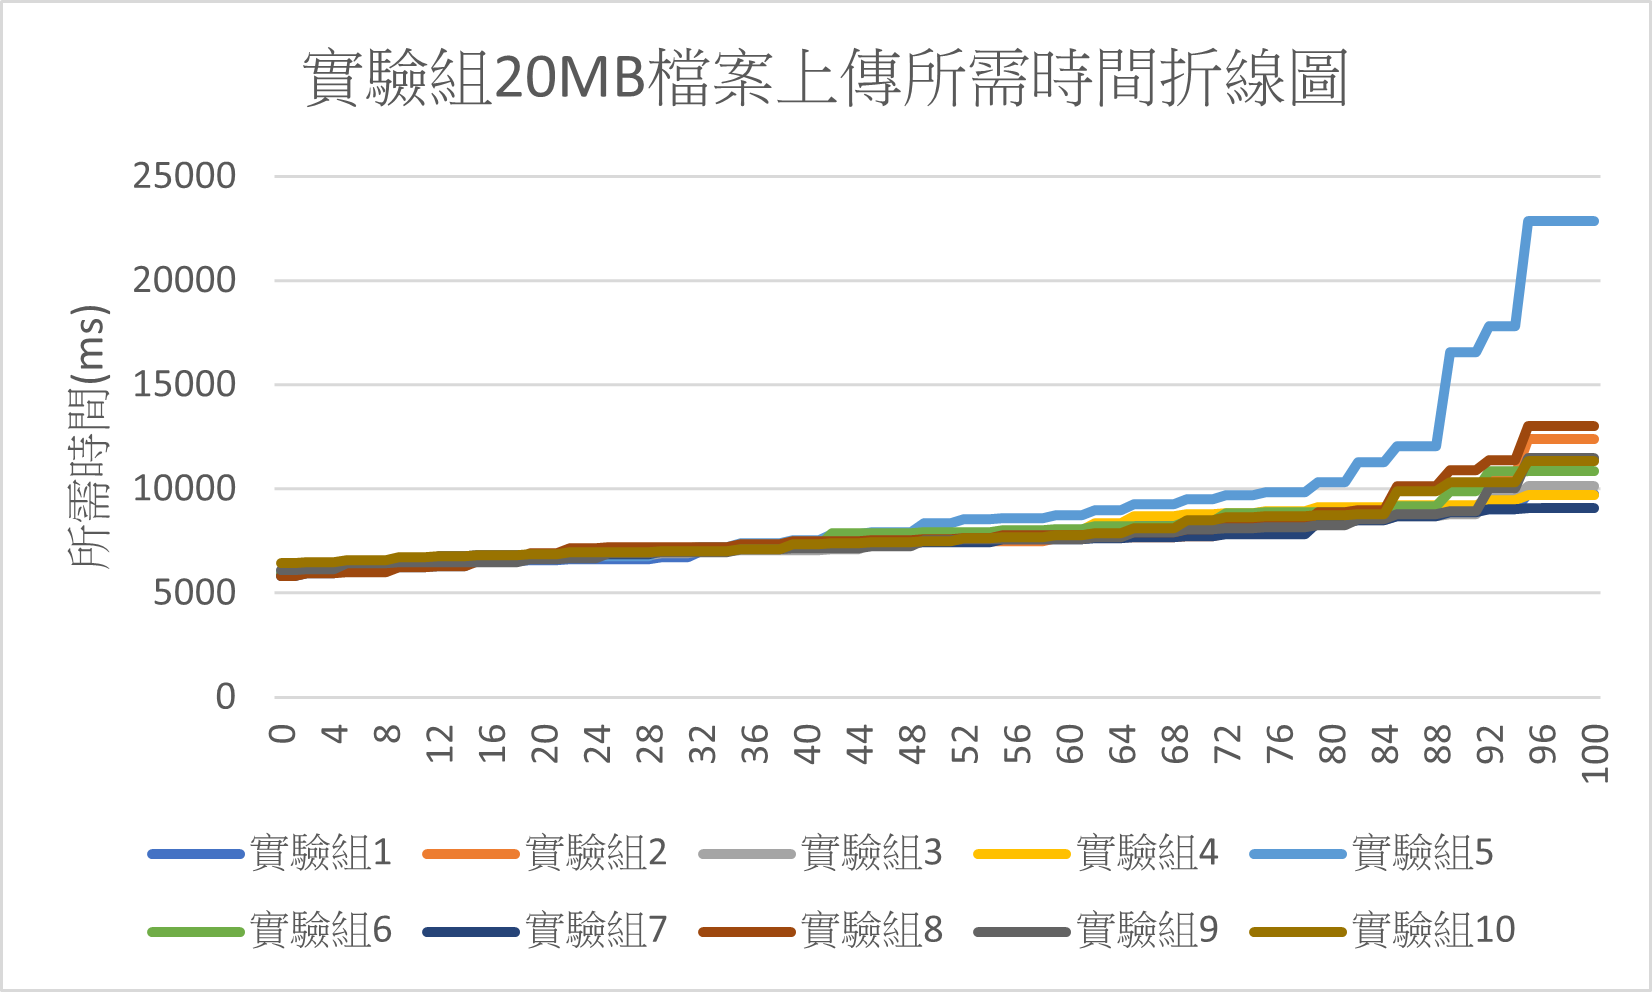
\includegraphics[scale=0.55]{實驗組20MB檔案上傳所需時間折線圖.png}
\caption{實驗組20MB檔案上傳所需時間折線圖}
\end{figure}

\begin{figure}[h]
\centering
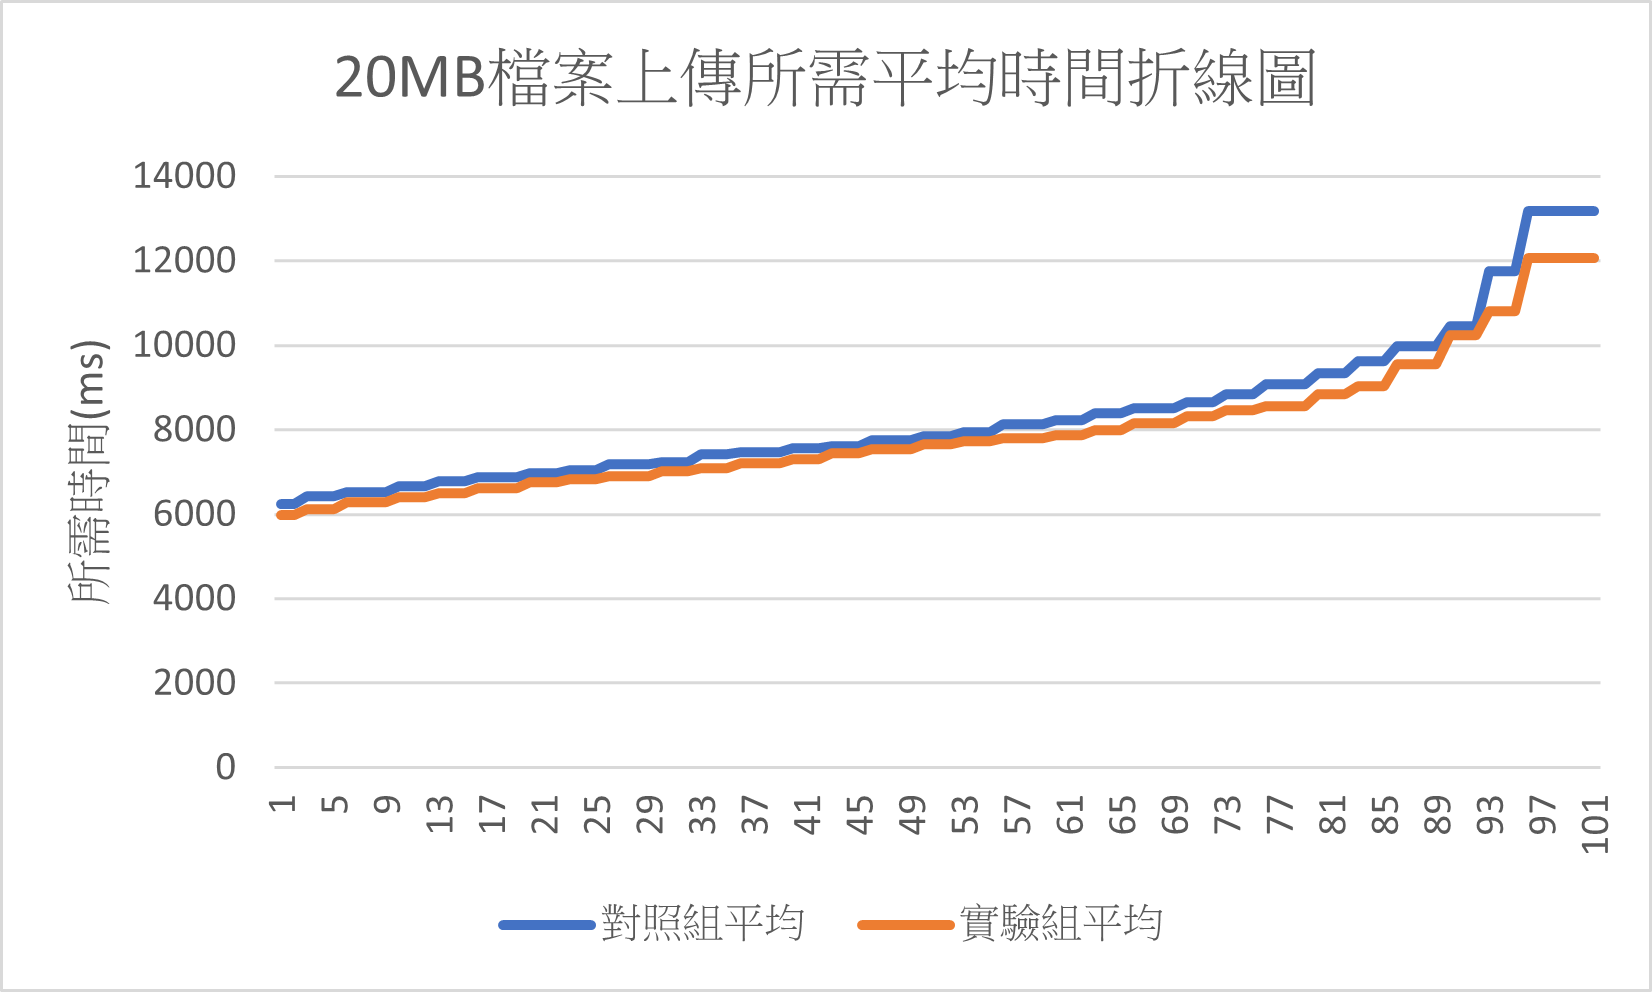
\includegraphics[scale=0.55]{20MB檔案上傳所需平均時間折線圖.png}
\caption{20MB檔案上傳所需平均時間折線圖}
\end{figure}\par
綜合上三圖所示,研究結果可以發現,實驗組在20MB大檔案上傳的表現仍然比對照組略為有效率,所需時間較短,且處理時間亦是相對穩定。\par
實驗過後,結果發現:本系統之效能在表現上不但跟原始資料儲存方式相近,甚至有些數據比起原始還要快,足見本系統具有實際商業使用之可能性。\par

\section{討論}
研究者認為,本研究提出之系統能表現得比原儲存方式更好,是因為每個資料庫所需儲存的內容變少,變成分散到不同的資料庫儲存,如此一來儲存的速度能有所提升。而系統能增加安全性之原因為資料分割以後,部分的密文因為是不完整的,且金鑰是客戶端所傳送的,更難取得,因此欲還原成原本未加密前的資料內容,是十分困難的。\par
本系統中的分割資料演算法因為是依序儲存於資料庫中,倘若得到全部資料庫的內容以後,就可以輕易地將資料合併,得到密文後,如果有心人士有極強的算力資源或背後有龐大的資金支持,那麼就有可能透過暴力破解將資料解密,如果未來能夠將分割資料的演算法增強,用其將分割後的資料依照某一方式,儲存到不同的資料庫中,那麼資料的安全性定會更上一層樓。\par

\section{結論與未來展望}
\subsection{結論}
現今網路快速地發展,每個人的資料在網路上不斷的流通,倘若無法做好資安防護,將資料保護好,肯定是一大問題。\par
透過此研究對於本系統的API進行壓力測試過後,發現在一定的使用者數量下,整套系統都可以保持高效率、高穩定的運作,處理時間都在1秒以下,惟當同時連線的使用者數變多時,本系統才會需要較久的處理時間,大部分的狀況下,本系統的處理時間皆與一般使用加密算法加密過後再存入資料庫中的時間差不多(差距在100毫秒下)甚至有些測試資料,本系統會表現得比原本既有的儲存方式來的更好,基本上可以滿足一般小型網站正常的使用,並不會造成太大的問題,如此一來,僅需犧牲一些效率,就能增加資料的安全性。\par
對於一般網路應用程式開發者,可以採用本研究提出之系統,解決目前單一資料庫被攻破,所有資料即會外洩的問題,如:電商網站在儲存使用者之個人資料時,可以採用本系統作為後端的資料庫管理程式,除了降低資安風險,亦可確保資料庫的穩定性,又或者是企業內部要儲存企業商業機密時,可採用本系統,確保資料安全無虞等,本系統在實際運用上可以為開發者及企業降低不少維護資訊安全的時間。\par
\subsection{貢獻}
本研究使用了Docker和Flask等軟體時做了提出的系統,並驗證了實際使用的可行性,此外,系統中的加密分割儲存技術是市面上未曾出現過的儲存方法,為本研究之創新。透過壓力測試,驗證了該系統之商業運用的可行性。 \par
本研究之專案原始碼將開源於Github上,讓對於此領域有興趣的相關研究人員研究,可以一同維護專案,共同為資安領域奉獻心力,同時也讓企業或個人開發者在部屬本系統時,能更安心、更便利的部屬。網址:\url{https://github.com/DDBMS/} \par

\subsection{未來展望}
本研究目前使用的是MySQL作為資料儲存後端,希望為來能夠支援更多的儲存後端,例如:加入區塊鍊技術,提供公開、不可竄改之資料儲存,或者是研發更加的儲存技術,思考將儲存效率提高之方法。\par
未來研究建議希望能將系統架構再做修改,若資料並非是機密資料,可讓此套系統架構應用到公開的不可竄改資料,讓Database Group的每個節點都變成一備選之DDBMS,當系統中的DDBMS失靈時,任一節點皆可提升變成DDBMS,如此一來可使系統變得更加「分散式」,不會有過於中心化之虞。\par

\bibliographystyle{plain}
\bibliography{references}

\end{document}
